% Generated by scripts/supp_tex.py from scripts/supp/a_implementation.py.
% Do not edit: edit the module, which also builds the PDF version.

\section{Test settings, implementation and reproducibility}
\label{supp:a_implementation}

\subsection{What this section covers}

This section is the recipe and the protocol: the released codec the work starts from and the exact file it is, the test set, the conventions every decibel is measured under, every module with its shape and its parameter count, the training configuration with a column naming where each choice was measured, the hardware, the seeds and what varies between two runs of one command. Numbers are not repeated across sections; where a quantity belongs to a later one, this section names it and stops. One fact governs the rest and is stated here rather than buried: the checkpoint every headline number comes from has seen the training set exactly once, and A.10 reports how much the numbers move with a second pass.

\subsection{Test settings: the released codec, and what is frozen}

There is no traditional-codec invocation in this work and none is needed. The axis measured here is decoder-side compute against a fixed learned decoder, on a bitstream that decoder produced, so the anchor is a checkpoint rather than a command line, and the released codec's own standing against VTM is published with it. That checkpoint is identified by content and not by path, because the released file is a bare state dict carrying no epoch, no optimiser and no step, so a path plus a hash is the whole of its provenance.

{\small The anchor is ~/DCVC/checkpoints/cvpr2026\_image.pth.tar, sha256 b3b900de23f30e4fc437010ddffe6a5413a56d6cfd97fb6235adbcd2b6973302, recorded with that reading in results/dmc\_ld\_recon\_audit.json.}

The codec is imported rather than reimplemented: flexuf/model.py sets DCVC\_ROOT to the DCVC checkout and imports src.models.image\_model.DMCI from it, so the entropy model, the hyperprior, the quantisation-step tables and the 64 quality indices are the released code running unmodified. Our decoder is those weights rearranged: an opening upsampling block, 12 DepthConvBlocks at C = 384 channels and a head that pixel-shuffles back to RGB, with the 12 blocks grouped into K = 6 exits of b = 2 blocks each and the first j = 2 groups running once over the whole frame before the decode splits into tiles. Exits 0 and 1 therefore lie below the split and cannot be selected; the four reachable exits are 2 to 5.

The encoder is frozen for the whole of training, and that is asserted rather than assumed: scripts/signalled\_curve.py compares our encoder state dict against the released one tensor by tensor and requires the largest absolute difference to be exactly zero before a single frame is measured. A trained decoder therefore consumes byte for byte the stream the released encoder produces, the bit rate is identical by construction, and the whole of the measured difference is decoder-side.

\subsection{The test set, and what tiling does to it}

\begin{table}[t]
\centering
\resizebox{\columnwidth}{!}{%
\begin{tabular}{lrrrrr}
\toprule
class & sequences & resolution & padded to & tiles & added px \\
\midrule
UVG & 7 & 1920x1080 & 2048$\times$1280 & 40 & 26.4\% \\
MCL-JCV & 30 & 1920x1080 & 2048$\times$1280 & 40 & 26.4\% \\
HEVC B & 5 & 1920x1080 & 2048$\times$1280 & 40 & 26.4\% \\
HEVC E & 3 & 1280x720 & 1280$\times$768 & 15 & 6.7\% \\
HEVC C & 4 & 832x480 & 1024$\times$512 & 8 & 31.3\% \\
HEVC D & 4 & 416x240 & 512$\times$256 & 2 & 31.3\% \\
all & 53 &  &  &  &  \\
\bottomrule
\end{tabular}}
\caption{The test set, and what tiling does to each resolution. Take from it that granularity is not constant across the set: a 1080p frame carries 40 tiles for the allocation to work with and a 416$\times$240 frame carries two, and the small classes also pay the most padding. That single fact explains most of the per-class spread reported in section D.}
\end{table}

{\small Sources: results/per\_class\_RECIPE512.json for the class membership and tile counts, results/tile\_definition.json for the padded sizes; both on runs/RECIPE512/ckpt\_PAPER.pth.tar. The sequences are UVG [23], MCL-JCV [24] and HEVC classes B, C, D and E [7]; the full list of \NumSeq names is recorded in the measured field of results/signalled\_RECIPE512\_ctc53.json, with not\_measured empty.}

Frames are the leading frames of each sequence, taken consecutively. The headline file uses two frames on each of the \NumSeq sequences of Table 1, so 106 frames; the routed, rate-rank and partial signalling tables use one. Every results file records frames\_per\_seq and every table in this supplement states it. No frame is dropped and no sequence excluded: the not\_measured field of every curve file is empty.

Border padding is an \emph{estimator} of the unseen neighbour, and the seam is its error, so the four rules below are four estimators compared on the same frames with early exit switched off, leaving tiling as the only difference from a full-frame decode.

\begin{table}[t]
\centering
\resizebox{\columnwidth}{!}{\begin{tabular}{lrrr}
\toprule
Border estimator & $q0$ & $q32$ & $q63$ \\
\midrule
Zeros (stock) & 0.126 & 0.287 & 0.677 \\
Replicate & \textbf{0.071} & \textbf{0.123} & \textbf{0.218} \\
Linear extrap. & 0.198 & 0.286 & 0.384 \\
AR(1) per channel~\cite{arls} & 0.061 & 0.107 & 0.197 \\
\bottomrule
\end{tabular}
}
\caption{\textbf{Border estimators}, dB below the released decoder on the same latent, 256 px tiles, full CTC, with every tile at full depth. Lower is better. The ordering is not the obvious one. Replication, a zero-order hold, beats linear extrapolation by a wide margin, because extrapolating the local gradient past a boundary amplifies whatever noise sits on that boundary and assuming local constancy does not: \SeamLinearHigh dB against \SeamReplHigh dB at q63. The fitted per-channel AR(1) rule wins on quality, reaching \SeamArlsHigh dB, and loses on cost at +10.7\% of decode wall-clock, which against a 0.1 dB budget does not close; section H carries that verdict in full.}
\end{table}

{\small results/ctc\_seam\_p256.json, generated into paper/tables/padding.tex by scripts/make\_paper\_tables.py. The shipped configuration is replicate padding.}

Tile size is the other half of what tiling costs, and it is free in arithmetic: a tiled decode's multiply-accumulate count does not depend on the tile side at all, because every tile runs the same graph and the tiles partition the same feature map. What the side buys is granularity for the allocation, and what it costs is seam. The two sides we have measured are below.

\begin{table}[t]
\centering
\resizebox{\columnwidth}{!}{\begin{tabular}{lrrr}
\toprule
Estimator, $q63$ & 128\,px & 256\,px & ratio \\
\midrule
zeros & 1.249 & 0.677 & $\times$0.54 \\
replicate & 0.372 & 0.218 & $\times$0.58 \\
arls & 0.332 & 0.197 & $\times$0.59 \\
\bottomrule
\end{tabular}
}
\caption{\textbf{Tile size, at q63.} dB below the released decoder with every tile at full depth, so this is tiling penalty and nothing else. Doubling the side roughly halves the penalty, which is what a perimeter-driven error predicts, and it costs no computation. Against that, 256 px gives a 1080p frame 40 tiles to allocate across and 128 px gives it 160; section H reports what happened when we tried to spend that granularity.}
\end{table}

{\small results/ctc\_seam\_p256.json and results/ctc\_seam\_p128.json, generated into paper/tables/tilesize.tex by scripts/make\_paper\_tables.py. The two tile sizes come from separate training runs, which is the confound section H states.}

\subsection{The measurement conventions}

\begin{itemize}\itemsep1pt
\item \textbf{Colour.} Sources are YUV 4:2:0, 8 bit, converted to 4:4:4, divided by 255 and shifted by $-$0.5 for the network. PSNR is the released codec's own metric, (6$\cdot$Y + U + V)/8, computed after converting the reconstruction back to 4:2:0 on the 0 to 255 scale. Measuring in 4:4:4 would compare against a chroma upsample of the source rather than the source, and would report a chroma PSNR no published DCVC-UF number could be compared with.
\item \textbf{Padding.} Frames are padded by replication, bottom and right only, to a whole number of tiles; results/tile\_definition.json records the site as the RGB frame before the encoder and the mode as "replicate, bottom and right only: F.pad(x, (0, pw, 0, ph))". The stock codec aligns to 16, which is enough for the transform and not for a tile grid. Rate is charged on the true pixel count and PSNR computed after cropping back, so padding can cost and cannot flatter, and it does cost: a tile containing replicated rows gives up about twice the quality of one that does not.
\item \textbf{Decibels.} The main paper's protocol box fixes the convention; what it does not say is that pooling all tiles into one mean squared error first, which is the other live convention, moves the answer by about a third of a 0.1 dB budget. Section E measures that gap. No table here mixes the two and every table says which it is on.
\item \textbf{A second metric.} MS-SSIM is reported beside PSNR at the operating point, computed as Wang et al. 2003, 5 scales, 11-tap Gaussian sigma 1.5, valid region, luma plane in 4:2:0 on 0..255. The implementation is self-checked at start-up: identical inputs score 1.000000 and a 3$\times$3 box blur scores 0.7797, both recorded in results/supp\_opquality\_PAPER.json.
\item \textbf{The map is billed.} The exit map is entropy coded from a per-frame histogram and its cost added to the rate before any saving is computed: 79 to 95 bits per frame at the 0.1 dB budget, at most 9.09e-05 bpp. Every row records map\_bits and the bpp it added.
\item \textbf{The reference.} The released decoder re-expressed in the same ladder and selected by K, so a K = 12 run cannot be quoted against the K = 6 remap.
\end{itemize}

{\small The padding figure and the second metric are both from results/supp\_opquality\_PAPER.json on the pinned checkpoint, 53 sequences at the 0.1 dB operating point: mean per-tile penalty 0.260 dB over the 547 tiles containing replicated rows against 0.121 dB over the 1,218 that do not, at q0. The map-bit range is from results/signalled\_RECIPE512\_ctc53.json, field map\_bits.}

Two limits belong beside that list. Sweeping a multiplier reaches only the lower convex hull of the achievable set [26, 27], so a budget falling in a gap of the hull is met at the nearest reachable point; every row carries a reachability flag and a floor, and rows whose floor already exceeds the budget are reported as unreachable rather than dropped. And 0.1 dB is a reporting convention, not a perceptual threshold. Subjective work measures the smallest noticeable change in quantisation parameter or in a video quality metric, not in tenths of a decibel of PSNR, so nothing published licenses a claim that 0.1 dB is invisible; 0.3 dB and 0.5 dB are reported beside it so that the choice carries no weight.

\subsection{The ladder, module by module}

\begin{table}[t]
\centering
\resizebox{\columnwidth}{!}{%
\begin{tabular}{lrrrr}
\toprule
module & runs & in $\rightarrow$ out & params & share \\
\midrule
upsample & frame & 256 $\rightarrow$ 384, $\times$2 & 1,431,936 & 10.1 \\
groups 0 to 1, stem & frame & 384 $\rightarrow$ 384 & 4,154,880 & 29.2 \\
groups 2 to 5, routable & tile & 384 $\rightarrow$ 384 & 8,309,760 & 58.4 \\
one DepthConvBlock & tile & 384 $\rightarrow$ 384 & 1,038,720 & 7.3 \\
adapters 0 to 3, FFN & tile, at its exit & 384 $\rightarrow$ 1536 $\rightarrow$ 384 & 739,200 & 5.2 \\
adapter 4, 1$\times$1 & tile, at its exit & 384 $\rightarrow$ 384 & 147,840 & 1.0 \\
seam repair, grid & after stitching & 384 $\rightarrow$ 384 & 152,704 & 1.1 \\
head, PixelShuffle 8 & frame & 384 $\rightarrow$ 192 $\rightarrow$ 3 & 335,232 & 2.4 \\
router head (B) & tile & 161 $\rightarrow$ 6 & 144,024 & 1.0 \\
decoder, released &  &  & 14,231,808 & 100.0 \\
decoder, ours &  &  & 3,257,344 & +22.9 \\
encoder, frozen & encode &  & 27,956,246 & 196 \\
\bottomrule
\end{tabular}}
\caption{Where every module sits, what shape it is and what it weighs, with the last column as a percentage of the released decoder's own parameters; adapter rows are per adapter and group rows cover the whole run of groups. Take from it three things. The ladder adds 22.9\% to the decoder's parameters, almost all of it in the four feed-forward adapters. Of that, 1,478,400 parameters can never run, because at j = 2 the decoder clamps every exit to at least 2 and adapters 0 and 1 are unreachable; they still take gradient from the distillation term, which taps every exit, and dropping them would forfeit the ability to re-run the same checkpoint at another split depth. And the frozen encoder is larger than the whole decoder, which is why an encoder-side search is the expensive half of this system and a decoder-side one is not.}
\end{table}

{\small Source: results/supp\_module\_shapes.json, derived by scripts/module\_shapes.py from the state dict of runs/RECIPE512/ckpt\_PAPER.pth.tar (md5 daa3760937ea0bd8) on the CPU. Parameter counts are tensor sizes read straight from the state dict. The same file also carries each module's multiply-accumulates per feature pixel, and the three aggregate shares that fall out of them, 8.16\% for the upsample, 89.44\% for the twelve-block trunk and 2.40\% for the head, reproduce the forward-hook audit of results/mac\_audit.json to four decimals. Section B prices the decode module by module and derives the per-exit cost; none of that is repeated here.}

One initialisation detail behind the seam-repair row of Table 4 is load-bearing and is not visible in the arithmetic. The pass multiplies its correction by a learned gate indexed by position within a tile, a 32$\times$32 array of scalars shared across all 384 channels, and that gate starts as a decaying function of the distance to the nearest tile edge. At step zero the module therefore already knows where the seams are and training refines rather than discovers, while its output convolution is still zero, so the whole module is exactly the identity and the warm-start controls of A.9 still hold.

\begin{figure}[t]
\centering
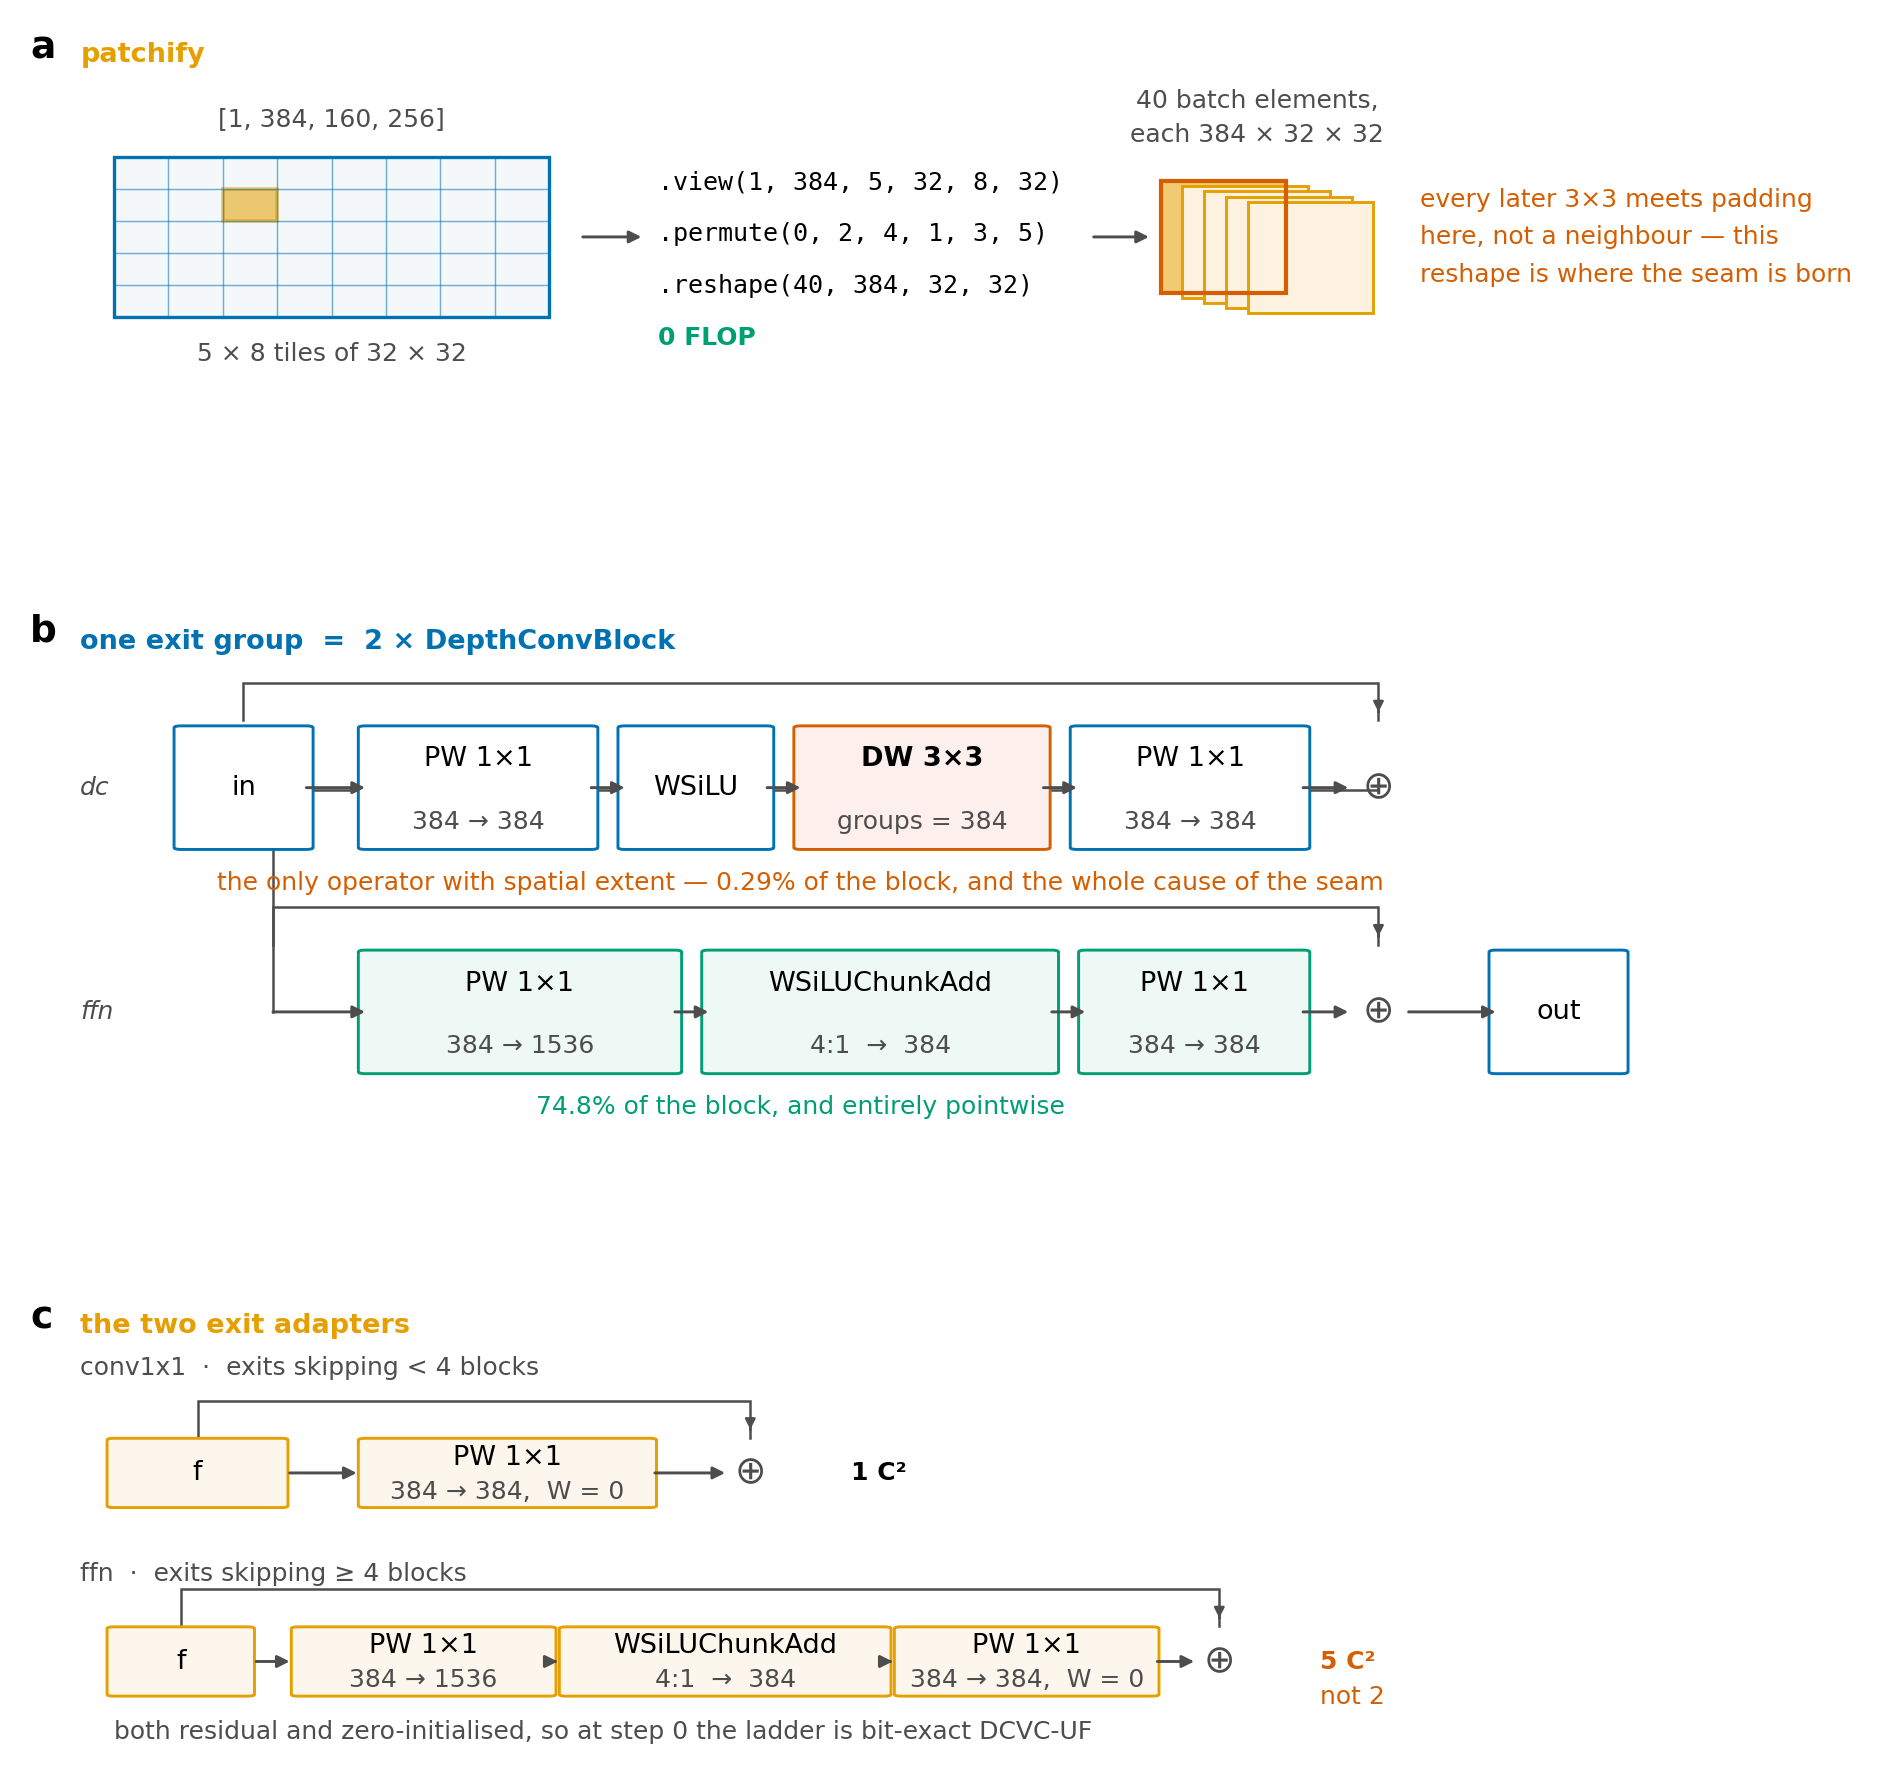
\includegraphics[width=\columnwidth]{figures/pipeline_detail.png}
\caption{\textbf{The three pieces a reader has to re-implement.} \textbf{a}, patchify is a pure reshape and costs nothing, and it is where both the seam and every operation of saving come from. \textbf{b}, one exit group is two DepthConvBlocks, whose only operator with spatial extent is a single 3$\times$3 depthwise worth 0.33\% of the block (9C of the block's 7C$^2$ + 9C, results/mac\_audit.json), so an early exit gives up almost purely pointwise capacity. \textbf{c}, the two adapters that replace it, both residual and both zero-initialised. Shapes are those of a 1080p frame padded to 2048$\times$1280 and split into 40 tiles.}
\end{figure}

\begin{figure}[t]
\centering
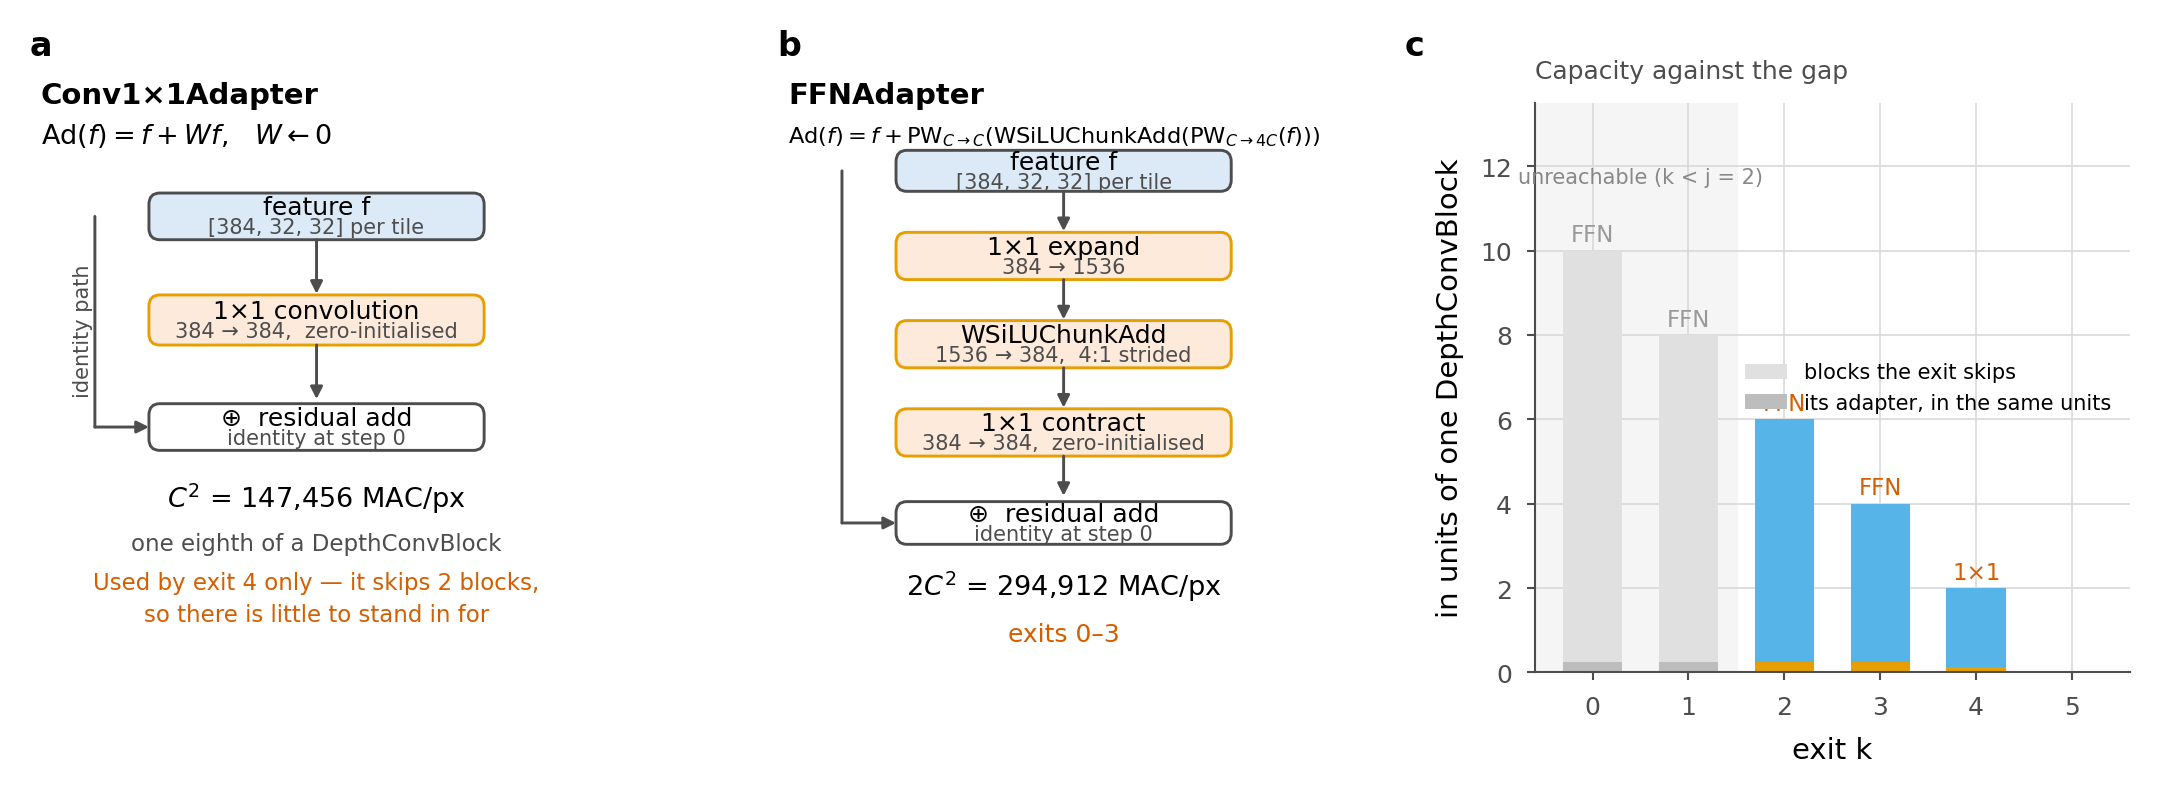
\includegraphics[width=\columnwidth]{figures/adapters.png}
\caption{\textbf{Inside an exit adapter.} \textbf{a}, one DepthConvBlock and the two adapters, drawn to scale: bar length is a share of the block, bar height the channel width written. Neither adapter contains the block's only 3$\times$3 (the hairline rule), so neither adds receptive field or seam penalty, which is the design constraint the seam measurement imposes. \textbf{b}, blocks skipped per exit, coloured by adapter; the rule switches to the FFN at four skipped blocks. Lengths are counted with hooks off the modules themselves.}
\end{figure}

What the adapters are worth is measured rather than argued, and the measurement is available because the identity is exactly what they were initialised to. Setting each adapter back to that identity leaves the ladder otherwise untouched, so the difference is what training put into them.

\begin{table}[t]
\centering
\resizebox{\columnwidth}{!}{\begin{tabular}{lrrrrrr}
\toprule
& \multicolumn{2}{c}{$q0$} & \multicolumn{2}{c}{$q32$} & \multicolumn{2}{c}{$q63$} \\
Exit & with & without & with & without & with & without \\
\midrule
2 & 0.177 & 2.065 & 0.228 & 2.884 & 0.297 & 4.398 \\
3 & 0.089 & 1.023 & 0.123 & 1.772 & 0.151 & 3.054 \\
4 & 0.056 & 0.416 & 0.077 & 0.574 & 0.084 & 0.853 \\
5 $^{\dagger}$ & 0.036 & 0.036 & 0.048 & 0.048 & 0.056 & 0.056 \\
\bottomrule
\end{tabular}
}
\caption{\textbf{What the adapters are worth.} dB below the released decoder with every tile at that exit, with the trained adapters and with each set back to the identity it was initialised to. The deepest exit has no adapter by construction and is the control, and it moves by exactly zero. Without the adapters the shallowest exit costs \AdapterNoneHigh dB at q63, forty-four times the working budget, and the adapter buys \AdapterGainHigh dB of that back.}
\end{table}

{\small results/adapter\_ablation.json, on runs/RECIPE512/ckpt\_PAPER.pth.tar, generated into paper/tables/adapters\_ablation.tex by scripts/make\_paper\_tables.py.}

\subsection{Tiles, and the exit clamp}

patchify is a view, a permute and a reshape with no arithmetic at all: a feature map of shape [1, 384, 160, 256] becomes 40 batch elements of [384, 32, 32], as panel a of Figure 1 shows. Tile order is row major, which is what the exit map is indexed by and what flexuf/eval.py reproduces with the same permutation when it measures per-tile error. One tile is 256 px of RGB, 32 px of feature map and 16 px of latent, at 16 pixels per latent position. patchify asserts divisibility rather than padding: an unpadded 1080p frame gives a 40$\times$40 feature map that is not divisible by 32, and the run stops instead of producing a ragged last row.

The clamp is the most consequential line in the decoder. forward() applies exit\_map.clamp(min = j, max = K $-$ 1) before the per-tile loop, so a map naming exit 0 at j = 2 runs group 2 and wears exit 2's adapter. Four separate places have to apply that same clamp, and getting any of them wrong is silent rather than loud, which is why they are listed rather than described.

\begin{table}[t]
\centering
\resizebox{\columnwidth}{!}{%
\begin{tabular}{lr}
\toprule
file and function & what it does \\
\midrule
decoder.py, forward & clamps the map to [j, K$-$1] before the per-tile loop \\
cost.py, exit\_costs & charges max(k, j) blocks, and bills the adapter the clamped exit wears rather than the one the map names \\
eval.py, tiled\_exit\_mses & fills the columns below j with the decode at exit j, so an argmin over all K lands on a reachable choice \\
head2.py, forward and oracle\_ce\_loss & masks the logits below the split depth with $-$inf, and clamps the oracle label to the same bound \\
\bottomrule
\end{tabular}}
\caption{The exit clamp, and the four places that have to repeat it. A clamp in the decoder without the matching clamp in the cost model bills a shallow map for compute it never ran, which is a saving no meter agrees with. The mask in the router is $-$inf and not a large negative constant, because nothing in a cross-entropy penalises a common offset added to every logit, so a finite mask can stop being the smallest entry in its row.}
\end{table}

{\small Source: the four files named in the first column, under flexuf/.}

\subsection{The deployed decode, and how training differs from it}

\begin{table}[t]
\centering
\resizebox{\columnwidth}{!}{%
\begin{tabular}{l}
\toprule
\textbf{input} latent y, quantisation step q, exit map m \\
\&nbsp;1\&nbsp; f = upsample(y) \\
\&nbsp;2\&nbsp; \textbf{for} g = 0 … j$-$1: f = groups[g](f)   \emph{frame, no borders} \\
\&nbsp;3\&nbsp; tiles, nh, nw = patchify(f, 32)   \emph{reshape, 0 MAC} \\
\&nbsp;4\&nbsp; m = clamp(m, j, K$-$1)   \emph{below j cannot run} \\
\&nbsp;5\&nbsp; active = all tiles; work = tiles \\
\&nbsp;6\&nbsp; \textbf{for} g = j … K$-$1: \\
    \&nbsp;7\&nbsp; work = groups[g](work)   \emph{borders meet padding} \\
    \&nbsp;8\&nbsp; leaving = active tiles whose m equals g \\
    \&nbsp;9\&nbsp; out = adapters[g](work[leaving])   \emph{raw if g = K$-$1} \\
    10\&nbsp; \textbf{if} training: out = out $\cdot$ gate[leaving] \\
    11\&nbsp; canvas[leaving] = out \\
    12\&nbsp; drop leaving from work and from active   \emph{the saving} \\
13\&nbsp; canvas = unpatchify(canvas, nh, nw) \\
14\&nbsp; canvas = canvas + G[r mod P, c mod P] $\cdot$ seam(canvas) \\
15\&nbsp; \textbf{return} pixel\_shuffle(head(canvas $\cdot$ q), 8) \\
\bottomrule
\end{tabular}}
\caption{The deployed routed decode, line for line. Take from it that line 12 is the entire saving: every group runs on fewer tiles than the last, and nothing else in the procedure is cheaper than a full decode. Line 10 is the only difference between training and inference, and it is numerically the identity.}
\end{table}

Line 10 of Table 7 deserves the space. A router trained jointly with the decoder needs gradient to reach its logits and an argmax blocks it, so the gate is p / p.detach() with p the selected exit's probability under a Gumbel-softmax relaxation: its value is exactly 1 and the reconstruction bit-identical to the deployed path, while its gradient is the straight-through estimator. At inference the gate is absent and the exit is a hard argmax or a transmitted symbol. That is the one place where the trained object and the shipped object are not the same computation.

A second execution path exists and is bit-identical. With sorted execution the tiles are ordered by depth with a stable argsort before line 6, so "still active at group g" becomes a contiguous prefix, every group is a slice rather than a masked gather, and the loop costs one host read instead of one synchronisation per group. Only the wall clock moves, by \WallSortedGain points, and section B reports it.

\subsection{The training data}

Training uses Open Images [22], fetched from the CVDF public mirror by scripts/fetch\_openimages.sh and prepared by scripts/prepare\_openimages.py into the flat layout DCVC-UF's own ImageFolder expects. Of 384,795 files scanned, 380,126 survive a minimum-side filter of 512 px, 4,669 are dropped as too small and 0 as unreadable. The filter is not cosmetic: the loader zero-pads any image smaller than the current crop, and an image that is half black border teaches the decoder to reconstruct black borders. Every 400th entry of the sorted survivor list is then held out, giving 512 validation images and 379,614 training images with no overlap, deterministically, so every run and every control sees the same held-out set.

Each sample is a random crop at the schedule's patch size with a random horizontal flip, converted to YCbCr, scaled to [0,1] and shifted by $-$0.5. One quality index is drawn uniformly over the 64 levels per sample and the matching multiplier comes from the log-spaced table running 10 to 2048, so one set of weights covers the whole rate range rather than a point on it. The crop is 512 px, which is what the released recipe's final phase asks for and also the smallest crop carrying more than one tile: at 256 px tiles a 512 px crop holds 4 and a 256 px crop holds one. A single tile has no border against a neighbour, so patched training at the smaller crop would train a configuration that cannot occur at inference. Evaluation uses a deterministic centre crop with no flip, because the loader's random crop swung one model between 29.54 and 30.58 dB at q0 across two runs of one command.

\subsection{The warm start, and the controls it asserts}

scripts/warmstart\_from\_release.py performs the rearrangement, and it is a key remap and nothing else: the opening upsample takes dec\_1[0], group g block i takes dec\_1[1 + g$\cdot$b + i], the head takes dec\_2, and the adapters and the seam-repair gate are new and zero-initialised. The encoder, hyperprior, entropy model and quantisation-step tables are copied verbatim. The transfer moves 398 tensors and creates 28 adapters at initialisation. Two controls follow from zero initialisation and both are asserted at every build rather than assumed: the deepest exit reproduces the released decoder with a largest absolute difference of 0.0, and every untrained exit equals the released decoder truncated at that depth, also 0.0. A third lives in the checkpoint loader, which tolerates a missing or extra tensor only under the adapter, seam-repair, pad-coefficient and router prefixes and raises otherwise; both sides of a tolerated mismatch are zero-initialised identities, so dropping one is exact rather than approximate.

\subsection{The training run}

\begin{figure}[t]
\centering
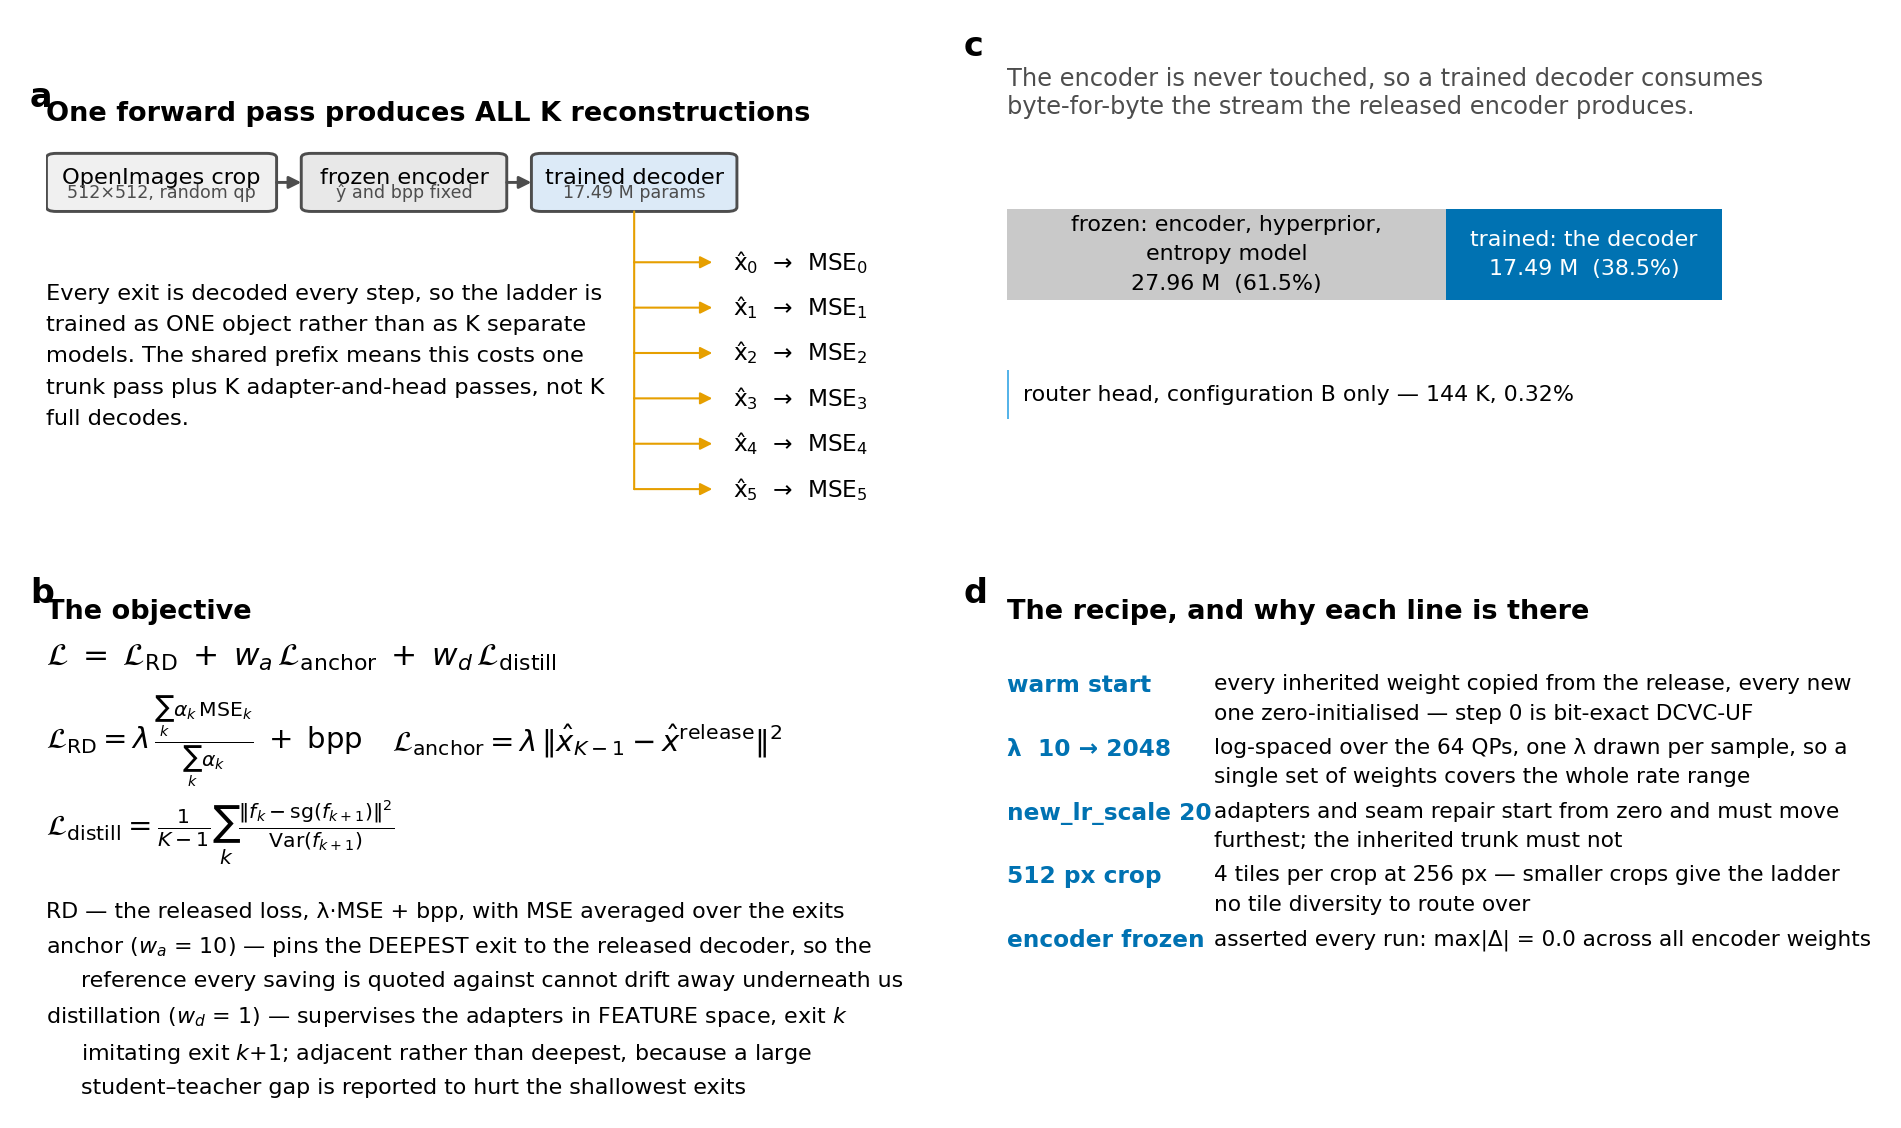
\includegraphics[width=\columnwidth]{figures/training_scheme.png}
\caption{\textbf{The training scheme.} \textbf{a}, one forward pass produces all K reconstructions, so the ladder is trained as one object. \textbf{b}, the three loss terms. \textbf{c}, the encoder is never touched. \textbf{d}, why each line of the recipe is there. The figure is a schematic drawn from the model definition; the parameter counts it carries are the ones tabulated in A.5.}
\end{figure}

The recipe, laid out in Figure 3, is Microsoft's own, applied at the point in their schedule that matches what we inherit. Their schedule is a 105-entry table of learning rate and crop size indexed by epoch, and the released weights are the output of its last entry, so applying entry zero would kick a converged codec with the from-scratch learning rate. The run enters at offset 99, inside their final 512 px phase at a learning rate of 1$\times$10$^{-5}$; all 852 records in the run's log carry that rate and that crop, which is the check that the offset did what it was meant to. Because the offset lands in the phase the experiment needs, no crop-size override is passed at all, where every other warm-started run here raises the crop floor by hand.

One deviation from a plain fine-tune is deliberate. The adapters and the seam-repair gate start at zero and have to move furthest, while the inherited trunk must not move at all if the deepest exit is to stay the released decoder, and the cost of choosing wrongly between them is measured: at the from-scratch rate the trunk drifts 0.20 dB of anchor at q32 in a single epoch. The new modules therefore get their own parameter group at 20 times the schedule's rate, selected by name prefix, with the multiplier re-applied whenever the schedule sets the base rate.

The loss has three terms. The rate-distortion term is the released loss, a multiplier times mean squared error plus bits per pixel, with the error averaged over the exits under fixed weights. The anchor term pins the deepest exit to a frozen copy of the released decoder, because every saving in the paper is quoted against that decoder and a reference drifting underneath the measurement makes the measurement meaningless. The distillation term supervises each adapter in feature space against the exit one step deeper, normalised by the teacher's own variance, following the adjacent-teacher form rather than the deepest-teacher form [15], since a large gap between student and teacher is reported to hurt the shallowest exits most. Gradients are clipped at a norm of 0.1 and a batch whose norm is not finite is dropped; across all 852 records the count of steps skipped for that reason is 0 and the median gradient norm is 0.273.

An epoch is 47,451 optimiser steps, which is 379,614 images at batch 8. The run logs every 200 steps and the median interval is 299.8 s, so a step costs about 1.5 s and an epoch about 19.8 hours. Training is fp32 throughout on a single NVIDIA RTX A6000 with eight data workers.

The pinned checkpoint is the first epoch boundary of a run whose launcher was given 16 epochs. Section H tabulates what the later checkpoints of this run and of its sibling measure at the same budget on the same frames; the one figure that belongs here is the floor, the quality given up before any tile exits early, which falls at every rate between the two epoch pins: it spans 0.0326 to 0.0659 dB at epoch 0 and 0.0295 to 0.0595 at epoch 1. No comparison in this paper between two runs at different epochs can be read as a comparison between two configurations, and where such a comparison appears it is labelled with both epochs. Nothing here extrapolates to a converged run.

{\small Floors from results/signalled\_RECIPE512\_ctc53.json (runs/RECIPE512/ckpt\_PAPER.pth.tar, epoch 0) and results/signalled\_RECIPE512\_e1.json (runs/RECIPE512/ckpt\_PIN\_e1.pth.tar, epoch 1), both 53 sequences at the 0.1 dB budget.}

\begin{equation}
\mathcal{L} = \mathcal{L}_{\mathrm{RD}} + w_{a}\,\mathcal{L}_{\mathrm{anchor}} + w_{d}\,\mathcal{L}_{\mathrm{distill}}.
\end{equation}

The distillation term is written in feature space and not in pixels because the head is a fixed map from feature to RGB, so matching the deeper feature is the stronger constraint, with 384 dense channels of target instead of three. Each exit imitates its neighbour, exit k following exit k+1, rather than the deepest exit.

One choice in the recipe matters more than the weights on those three terms. The adapters are trained \emph{through the tiled decode path they are deployed in}, which is what the train\_patched flag of the launcher above selects. Training them full frame and tiling only at inference loses 0.14 to 0.24 dB; training through the deployed path gains 0.51 to 0.90 dB, so the sign of the effect flips. A ladder that has never seen a seam does not know it has to compensate for one.

{\small Those two ranges are read from the run log recorded in DECISIONS.md for the warm-start and train\_patched comparisons; no file in results/ holds them.}

\subsection{Every hyperparameter, and where each was measured}

\begin{table}[t]
\centering
\resizebox{\columnwidth}{!}{%
\begin{tabular}{lrr}
\toprule
knob & value & searched, and where \\
\midrule
\textbf{ladder geometry} &  &  \\
exits K, blocks per exit b & 6, 2 & signalled\_BEST128 and signalled\_FINE12, at K = 12 \\
split depth j & 2 & supp\_seam\_vs\_split, j from 0 to 6 \\
RGB tile & 256 px & ctc\_seam\_p128 against ctc\_seam\_p256; tilesize\_adaptive \\
halo, latent and trunk & 2, 0 & no; the trunk halo was priced at 2.25$\times$ and rejected \\
adapter kind & scaled & adapter\_ablation \\
adapter expansion & 4 & no; the block's own 4:1 \\
seam repair & grid & supp\_seam\_vs\_split \\
tile padding & replicate & padding\_ablation: zeros, replicate, linear, arls \\
tile coupling & off & coupling\_ablation \\
full-frame head & on & the per-tile arm exists to measure it \\
\textbf{decoder training} &  &  \\
optimiser & AdamW & no; the released recipe's \\
schedule & 105 entries, at offset 99 & no; verified by scripts/verify\_recipe.py \\
learning rate & 1$\times$10$^{-5}$ & no; set by the schedule \\
multiplier, new modules & $\times$20 & no; set from one anchor-drift measurement \\
crop & 512 $\times$ 512 & no; set by the schedule \\
batch, workers, precision & 8, 8, fp32 & no \\
gradient clip & 0.1, non-finite dropped & no; released recipe's \\
multiplier range & 10 to 2048, 64 indices & no; released \\
quality index & uniform, per sample & no \\
anchor weight & 10 & two settings run; 10 kept \\
distillation & 1.0, adjacent & adjacent against deepest \\
auxiliary weight & 1.0, constant & no \\
training path & deployed tiled decode & against the full-frame arm \\
encoder & frozen & no; asserted at each evaluation \\
seed & none set & no; see A.15 \\
\textbf{router head, configuration B} &  &  \\
steps, batch, crop & 3,000, 6, 512 & no \\
learning rate, decay & 1$\times$10$^{-3}$ cosine, 1$\times$10$^{-4}$ & no \\
regret weight & 1.0 & no \\
seed & 0 & fixed, so the input ablation is comparable \\
live inputs & stem, latent, scales, qp & router\_ablation, six variants \\
\textbf{evaluation} &  &  \\
multiplier bisection & 60 halvings on [0, 1] & no \\
outer correction & 6 passes, tolerance 5e-4 dB & no \\
rate-rank bisection & 40 halvings & no \\
router bisection & on beta, bracket [$-$2e4, 2e4] & no \\
timing & 40 iterations after 20 of warm-up & protocol in section B \\
batch, when timing & 1 & supp\_latency\_batch, at 1, 2 and 4 \\
\bottomrule
\end{tabular}}
\caption{Every knob this work sets, its value, and whether it was searched. Take from it that almost nothing on the training side is tuned: the optimiser, the schedule, the clip, the crop and the multiplier range are the released recipe's, and the four settings that are ours exist to protect a property the measurement depends on rather than to improve a number. What was searched is the geometry, and the third column names the file in results/ that holds each comparison, so a reader can price the choice instead of taking it on trust.}
\end{table}

{\small Values come from scripts/launch\_recipe512.sh, train\_flexuf\_image.py, scripts/train\_router2.py and the four evaluation scripts; the third column names files in results/. The launcher's flags, without the two leading hyphens the shell needs, are: freeze\_encoder train\_patched epoch\_offset 99 new\_lr\_scale 20 anchor\_weight 10 seam\_repair grid adapter\_kind scaled distill\_weight 1.0 distill\_teacher adjacent lambdas 10 2048 batch\_size 8 n 8 e 16 num\_exits 6 split\_depth 2 latent\_patch 16 latent\_halo 2 aux\_weight 1.0 tile\_pad replicate.}

\subsection{Finding the operating point}

A budget is a quality target rather than a multiplier, so the multiplier has to be found, and it is found twice over: an inner bisection on a cheap table of per-tile distortions, and an outer correction against what a real decode delivers. The two levels exist because the table measures each tile with every other tile at the same exit, while a routed frame is mixed and a tile's border sees whatever depth its neighbour chose. The residual between them is small and nearly constant, so shifting the inner target by it converges in two or three passes, and each pass costs one decode per frame rather than one per bisection step.

Section G writes that search out line by line, with the shape each step returns. Three details of it change what the numbers mean. A rate whose floor exceeds its budget is written out with a reachability flag rather than dropped, so a saturated or unreachable row is visible instead of absent. The saving is measured and not modelled: a forward hook on every convolution and linear layer counts the multiply-accumulates the routed decode performed and divides by the same count for the released decode on the same latent, so the ratio needs no calibration constant and a module skipped by an early exit costs nothing because its hook never fires. The gap between model and meter is reported in every row: at the 0.1 dB budget it runs from 0.43 to 0.69 points, always in the direction of the model flattering us, and it is the measured column the paper quotes.

Two saving columns exist and only one is quoted. One divides by our own deepest exit, the other by the released decoder, and the released decoder is the denominator every claim is stated against; it is exactly 1 in the units of the cost table, so the seam-repair tax stays inside the figure it is supposed to be net of. The same two-level scheme with different constants runs in scripts/raterank\_curve.py, scripts/router\_curve.py and scripts/hybrid\_curve.py, whose constants Table 8 lists.

\subsection{What the work cost to produce}

\begin{table}[t]
\centering
\resizebox{\columnwidth}{!}{%
\begin{tabular}{lrr}
\toprule
item & cost & source \\
\midrule
one decoder epoch & 19.8 h on one A6000 & train\_log.jsonl \\
the pinned checkpoint & 1 epoch & ckpt\_PAPER records epoch 0 \\
the run so far & 3 epochs and 27,400 steps & train\_log.jsonl \\
one router head & 3,000 steps, 1.03 h & router\_ablation\_stem \\
encoder search, per frame & 4.52 decodes & supp\_encoder\_cost \\
decoder search, per frame & none & the map is signalled \\
\bottomrule
\end{tabular}}
\caption{What producing these numbers costs, priced rather than asserted. Take from it that the decoder is cheap to build and cheap to run, and that the whole of the allocation cost falls on the encoder, which already has the source and already runs an analysis pass. Sections B and F price the encoder-side search and the router heads against what they buy; this table only says what the work took.}
\end{table}

{\small Sources: results/router\_ablation\_stem.json for one head's wall\_s field, results/supp\_encoder\_cost\_PAPER.json for the search cost (pinned checkpoint, q63, 40 tiles, 15 iterations, one tiled decode at 114.9 ms). Decoder wall clock is from runs/RECIPE512/train\_log.jsonl; no file in results/ records it.}

\subsection{The pinned checkpoint, and what every table rests on}

Results are measured on runs/RECIPE512/ckpt\_PAPER.pth.tar, md5 daa3760937ea0bd89b89c555c2eefa88, which records epoch 0 inside itself and is byte identical to that run's ckpt\_epo0.pth.tar. The name exists because a filename is not a checkpoint here: a per-epoch watcher overwrites runs/*/ckpt\_eval.pth.tar as each epoch lands, so a results file naming that path names a file that no longer exists. scripts/make\_paper\_tables.py and scripts/check\_paper.py both hold the pinned name and, among candidates for one quantity, prefer a file whose own ckpt field records it, falling back to the most recently written; hand-written order breaks ties and nothing else.

Every run named in this document warm-starts from the released decoder through one of two key remaps, one per ladder size, and freezes the encoder, so all of them consume the identical bitstream and differ only in the ladder flags of A.11. They are compared only at labelled epochs, for the reason section H measures.

\begin{table}[t]
\centering
\resizebox{\columnwidth}{!}{%
\begin{tabular}{lrrr}
\toprule
results file & backs & checkpoint & seq$\times$fr \\
\midrule
signalled\_RECIPE512\_ctc53 & main results, complexity & pinned, e0 & 53$\times$1 \\
saturation\_RECIPE512\_ctc53 & operating range & pinned, e0 & 53 fr \\
static\_RECIPE512\_b01 & static controls & pinned, e0 & 53 \\
per\_class\_RECIPE512 & per class & pinned, e0 & 53 fr \\
router\_RECIPE512\_b01 & A against B & pinned, e0 & 53$\times$1 \\
router\_RECIPE512\_b03 & A against B & pinned, e0 & 53$\times$1 \\
raterank\_RECIPE512\_b01 & rate rank & pinned & 53$\times$1 \\
raterank\_RECIPE512\_b03 & rate rank & pinned & 53$\times$1 \\
raterank\_RECIPE512\_b05 & rate rank & R512/eval & 53$\times$1 \\
hybrid\_RECIPE512\_b01\_fixed & partial signalling & pinned & 53$\times$1 \\
hybrid\_raterank\_b01 & rate rank, second run & pinned & 53$\times$1 \\
hybrid\_v3\_b01 & rate rank, second run & R512/eval & 53$\times$1 \\
latency\_RECIPE512\_sorted & latency & R512/eval & - \\
router\_latency & operating range & R512/eval & - \\
adapter\_ablation & adapter ablation & R512/eval & 16 fr \\
combined\_RECIPE512\_b01 & blend & R512/eval & 53$\times$1 \\
hybrid\_RECIPE512\_b03\_fixed & macros only & R512/eval & 53$\times$1 \\
hybrid\_lorenz\_b01 & macros only & R512/eval & 53$\times$1 \\
coupling\_ablation & macros only & R512/eval & 16 fr \\
map\_transfer & macros only & R512/eval & - \\
band\_collapse & macros only & \emph{none} & - \\
band\_collapse\_BEST & macros only & \emph{none} & - \\
router\_retrain\_compare & macros only & \emph{none} & - \\
signalled\_BEST\_ctc53 & ladder configurations & BEST/eval, e1 & 53$\times$1 \\
signalled\_BEST128\_ctc53 & ladder configurations & BEST128/step, e1 & 53$\times$1 \\
signalled\_FINE12\_ctc53 & ladder configurations & FINE12/step, e1 & 53$\times$1 \\
ctc\_seam\_p256 & padding, tile size & \emph{none} & - \\
ctc\_seam\_p128 & tile size & \emph{none} & - \\
raterank\_BEST\_compare & rate rank, second run & \emph{none} & - \\
bdrate & BD-rate & \emph{none} & - \\
check\_paper & claim check & \emph{none} & - \\
\bottomrule
\end{tabular}}
\caption{Provenance of every generated table in the main paper. These are the 31 results files scripts/make\_paper\_tables.py reads, and the checkpoint column is read from each file at build time rather than typed. Take from it that 10 of the 31 are on the pinned checkpoint and the rest are not, so a reader comparing two rows of two different tables should check this column first. R512 abbreviates the run RECIPE512, "eval" is a per-epoch file the watcher overwrites in place, and "none" means the file records no checkpoint field.}
\end{table}

The pinned group of Table 10 carries the headline saving, the operating range, the per-class breakdown, the static controls and both routed configurations, so the paper's central claim rests on one epoch of one run measured consistently. Section H states what the rest of the column costs in reproducibility.

\subsection{Seeds, variation, and the interval that does exist}

No seed is set anywhere in the decoder's trainer. Four things vary between two runs of one command: the sampler is reshuffled every epoch from the global generator, the quality index is drawn per sample, the tiled training path draws a fresh random exit for every tile at every step, and cuDNN selects kernels by autotuning. The honest statement is that the recipe reproduces and the run does not, and this work has no repeated run of one configuration from which a training-side spread could be quoted. The router experiments are the exception and were built to be: every variant of the input ablation fixes seed 0 and shares architecture, parameter count, optimiser, image order and quality-index draws, so the only difference between them is which inputs the head may see, and their agreement figures carry a standard error across 1,200 frames.

\begin{table}[t]
\centering
\resizebox{\columnwidth}{!}{%
\begin{tabular}{lrrrrrr}
\toprule
quality index & mean & sd & min & median & max & worst sequence \\
\midrule
q0 & 32.70 & 7.51 & 6.04 & 35.89 & 39.12 & BQSquare \\
q16 & 28.81 & 10.60 & -0.95 & 31.67 & 39.12 & BQSquare \\
q32 & 24.58 & 12.04 & -0.95 & 26.10 & 39.12 & PartyScene \\
q48 & 22.40 & 11.75 & -0.95 & 23.54 & 39.12 & BlowingBubbles \\
q63 & 20.00 & 11.13 & -0.95 & 20.39 & 39.12 & RaceHorses \\
\bottomrule
\end{tabular}}
\caption{The interval this work can honestly report: saving in percent against the released decoder at the 0.1 dB budget, across the \NumSeq test sequences, on the pinned checkpoint. Take from it that the spread is content and not noise. It widens with rate, from a standard deviation of 7.5 points at q0 to 11.1 at q63, and the minimum turns negative at the high rates because a sequence whose tiles all stay at the deepest exit costs about 1\% more than the released decoder rather than less. This measures the test set, not the training draw, and is not a substitute for the run-to-run interval that does not exist.}
\end{table}

{\small Source: results/supp\_per\_sequence\_PAPER\_b010.json, the rows\_vs\_release block, computed from results/supp\_paper\_curve\_PAPER.json on runs/RECIPE512/ckpt\_PAPER.pth.tar. The file carries the same spread in our own deepest-exit denominator as well; the two differ by more than rounding and are never mixed.}

\begin{table}[t]
\centering
\resizebox{\columnwidth}{!}{%
\begin{tabular}{lrrr}
\toprule
quality index & path 1 & path 2 & gap \\
\midrule
q0 & 36.43 & 34.00 & 2.44 \\
q16 & 31.44 & 28.54 & 2.90 \\
q32 & 24.76 & 22.23 & 2.53 \\
q48 & 20.39 & 18.23 & 2.15 \\
q63 & 12.93 & 12.36 & 0.57 \\
\bottomrule
\end{tabular}}
\caption{Two implementations of the same quantity do not agree. Saving in percent at the 0.1 dB budget, computed by the curve-sweeping path and by the signalling path, which differ in how they pool distortion across tiles and frames. Take from it a floor on protocol sensitivity: the gap reaches 2.90 points, larger than several of the differences the paper draws conclusions from, so numbers from the two paths are never mixed inside one table.}
\end{table}

{\small Source: results/crosscheck\_paths.json. The file records no checkpoint field.}

Evaluation itself is deterministic once a checkpoint is fixed: the sequence list, the leading frames and the tile grid are all fixed and no crop is random. scripts/check\_paper.py re-reads \NumClaims numerical claims out of the paper's prose and checks each against the file it is supposed to come from. As recorded in results/check\_paper.json, 87 of them pass. All of them pass.

\subsection{Data, code and provenance}

\begin{itemize}\itemsep1pt
\item \textbf{Training images.} Open Images [22], from the CVDF public mirror named in scripts/fetch\_openimages.sh. The terms are the ones that mirror publishes and nothing here redistributes them.
\item \textbf{Test sequences.} UVG [23] from ultravideo.fi, MCL-JCV [24] and HEVC classes B, C and D from the public mirrors named in scripts/fetch\_mcljcv.sh and scripts/fetch\_hevc\_bcd.sh, and HEVC class E from media.xiph.org. Each fetch script records its source URL, and no sequence is re-encoded before it is measured.
\item \textbf{The released codec.} The DCVC-UF intra checkpoint [12], identified by sha256 in results/dmc\_ld\_recon\_audit.json and used under the licence its repository ships.
\item \textbf{Our code and checkpoints.} The trainer, the ladder, the cost model, the meter, the router and every evaluation script named here are in the repository this supplement is built from; the pinned checkpoint is identified by md5 in A.14.
\item \textbf{Human subjects.} None, which is why A.4 declines to claim that 0.1 dB is invisible.
\end{itemize}

